\chapter{Contexte général du projet}
\begin{onehalfspace}

\initial{L} e présent chapitre permet de situer le projet dans son contexte général, à travers, dans un premier temps, la présentation de l'organisme d'accueil, notamment l'entreprise Sayoo, de ses services et de son organisme interne.

\newpage


\section{Présentation de l'organisme d'accueil}

\textbf{Wireshark} est un DB programme qui permet d'écouter ce qui passe sur le réseau. Concrètement, Wireshark récupère les paquets réseau qui arrivent sur l'interface réseau et interprète leur contenu intelligemment pour les présenter de façon intuitive. Il permet ainsi de voir tous les paquets à destination de la carte réseau. C'est ce que l'on appelle un \textbf{Sniffer}.


\section{Cadre du projet}


\subsection{Présentation du projet}
 
la Société SAYOO tient à fournir des services de qualité à ses clients. Le projet consiste à améliorer le service \emph{ERP} fournit pour les entreprises.

Le service \emph{ERP} tient une importance capitale au sein de la société parce qu'il déploie des ressources importantes. Par ailleurs, toute relation avec une entreprise nécessite une rigueur et une grande attention.

Un client qui désire gérer les ressources de son entreprise  doit rencontrer un responsable de la clientèle de SAYOO pour spécifier ses besoins. Le responsable propose une version personnalisée de la suite \emph{Odoo} (anciennement \emph{Open ERP}) au client pour une gestion efficace. Par la suite, la société qui s'est déjà procurée  3 différents serveurs (Développement, Evaluation, Production) doit déployer une version de \emph{Odoo} sur le serveur de développement pour que les développeurs effectuent les premières personnalisations. Le client doit avoir accès au serveur Développement pour confirmer ou refuser. En cas de confirmation, l'administration doit déploier la version souhaitée sur le serveur production et conserver la version d'évaluation au cas d'une nouvelle mise à jour ou maintenance.Le serveur Evaluation a pour but de faire découvrir le client une version standard ou améliorée de la suite \emph{Odoo}.  

Pour une meilleure fiabilté, la société se procure 2 serveurs ( Déveleppoment, Production) par client. elle doit périodiquement effectuer des maintenances pour assurer la disponibilité de son service. Chaque client de la société se différentie seulement par sa personnalisation de la suite \emph{Odoo} donc les étapes de configuration sont redondantes pour tous les clients. Le temps de configuration et de déploiement reste important donc le client doit attendre pour accéder à son service après chaque maintenance. Les pré-requis de ce service sont relativement coûteux et affecte par conséquent le prix final du client.
  
















\subsection{Motivations}

Il va s'en dire que le processus de la provision des applications ERP pour les clients n'est pas optimale. D'où les motivations d'opter vers une solution cloud. Voici une liste des problèmes que rencontrent Sayoo lors du processus du déploiement actuel.

\begin{itemize}

\item La provision des instances Odoo est complètement manuelle. Ceci étant dit, quand un client demande une version de test d'Odoo par exemple, l'équipe de Sayoo est contrainte d'éxécuté une série d'étapes répétitives à partier de la commande, l'installation et la configuration su serveur jusqu'à la mise en place de l'application Odoo, configuration DNS, etc...;

\item Il y a un besoin récurrent des administrateurs qui doivent garder en permanence l'oeil sur applications des différents clients;

\item La supervision est quant à elle manuelle. En effet, au fur et à mesure que le nombre de clients augmente, l'administrateur doit ajouter les applications au système de supervision. Ceci est pénible, voire impossible, à suivre quand ,Ce qui rend le processus faible et non évolutive;

\item L'absense d'automatisme fait que l'équipe de Sayoo consacre la plupart du temps au tâches répétitives au lieu de le consacrer au développement et la personnalisation de l'application Odoo de chaque client. 

\item Il faut acheter un serveur pour chaque client pour y installer son application, ceci est un overkill pour atteindre le but. De plus, cela affecte le coùt de la solution.

\item Absence d'une architecture robuste qui peut garantir des éxigences non fonctionnelles énormes, à savoir la configurabilité, la haute disponibilité, la sécurité et la scalabilité. Ainsi, Sayoo ne garantie pas un SLA à ses clients;

\end{itemize}




\section{Objectifs du projet}
Ce projet vise principalement à améliorer le service ERP au sein de Sayoo par l'automatisation de certaines tâches notamment la configuration et le déploiement. L'objectif de ce projet est de déploier une architecture qui se caractérise par une haute disponibilité, une scalabilité selon les exigences et une sécurité sans faille. Par conséquent, cela revient à déployer une architecture \emph{cloud} qui répond aux exigences suivantes.
\begin{itemize}

\item Faciliter la configuration et le déploiement des instances Odoo pour les clients.

\item Eviter les tâches répétitives et faciliter la personnalisation de Odoo.

\item Réduire le coût en terme de temps et d'argent pour Sayoo.

\item Inclure un mécanisme de supervision fiable et évolutif.

\item Gérer aisement plusieurs clients en même temps.  
 






\section{Planification du projet}

Notre projet est loin d'être classique ainsi qu'il fait appel aux technologies non abordées le long de notre parcours scolaire. Du coup, une planification rigoureuse s'est imposé pour prévoir le déroulement du projet. Grâce aux réunions tenues avec les encadrants au sein de Sayoo, nous avons été éclairés sur les différentes étapes du projet ainsi que leur séquencement. Cela consistait en trois grandes étapes : la première est une phase de documentation dont les objectifs est de bien assimiler les nouvels concepts qui concernent le Cloud Computing, d'autre part de délimiter le périmètre du projet au niveau fonctionnel qu'au niveau technique. La seconde partie est consacrée à la conception de la solution, quant à la troisième étape, elle traite la mise en œuvre de la solution à travers la réalisation, test, et le déploiement.

Le stage a débuté le 23 mars pour une durée de 4 mois. Il en résulte le planning suivant :

\begin{figure}[H]
\centering
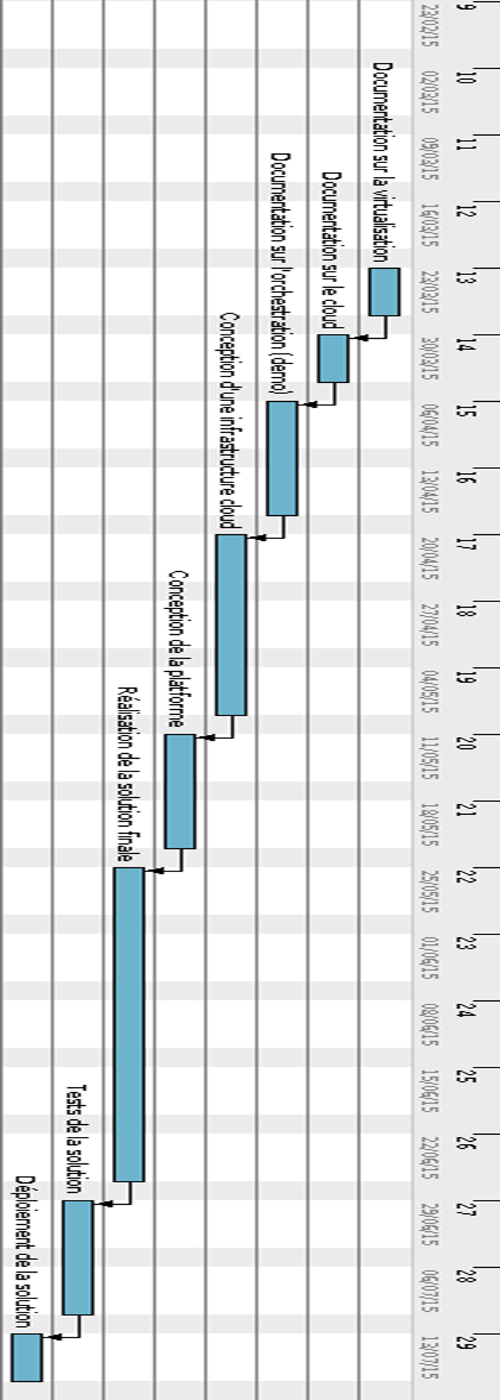
\includegraphics [scale=0.5]{chapitre1/assets/gantt.png}
\caption{Diagramme de Gantt}
\end{figure}


\end{onehalfspace}
